\documentclass[12pt,a4paper]{report}
\usepackage[utf8]{inputenc}
\usepackage[english,russian]{babel}
\usepackage{indentfirst}
\usepackage{pdfpages}
\usepackage{titlesec}
\usepackage{listings}
\usepackage{amsmath}

% Вставка картинки
\usepackage{graphicx}
\graphicspath{{schemes/}}
\DeclareGraphicsExtensions{.pdf,.png,.jpg}

\usepackage[14pt]{extsizes}

\newcommand{\hsp}{\hspace{20pt}}
\titleformat{\chapter}[hang]{\large\bfseries}{\thechapter{. }}{0pt}{\large\bfseries}
\titlelabel{hlabel-formati}
\titlespacing{\chapter}{42pt}{-20pt}{12pt}
\titleformat{\section}[hang]{\large\bfseries}{\thesection{. }}{0pt}{\large\bfseries}
\titlespacing{\section}{42pt}{12pt}{5pt plus 5pt}

% Отступ абзаца
\usepackage{indentfirst}
\setlength{\parindent}{1.5cm}

% Межстрочный интервал
\usepackage{setspace}
\onehalfspacing % интервал 1.5

\usepackage[left=3cm, right=1cm, top=2cm, bottom=2cm]{geometry}

\begin{document}
% Титульник
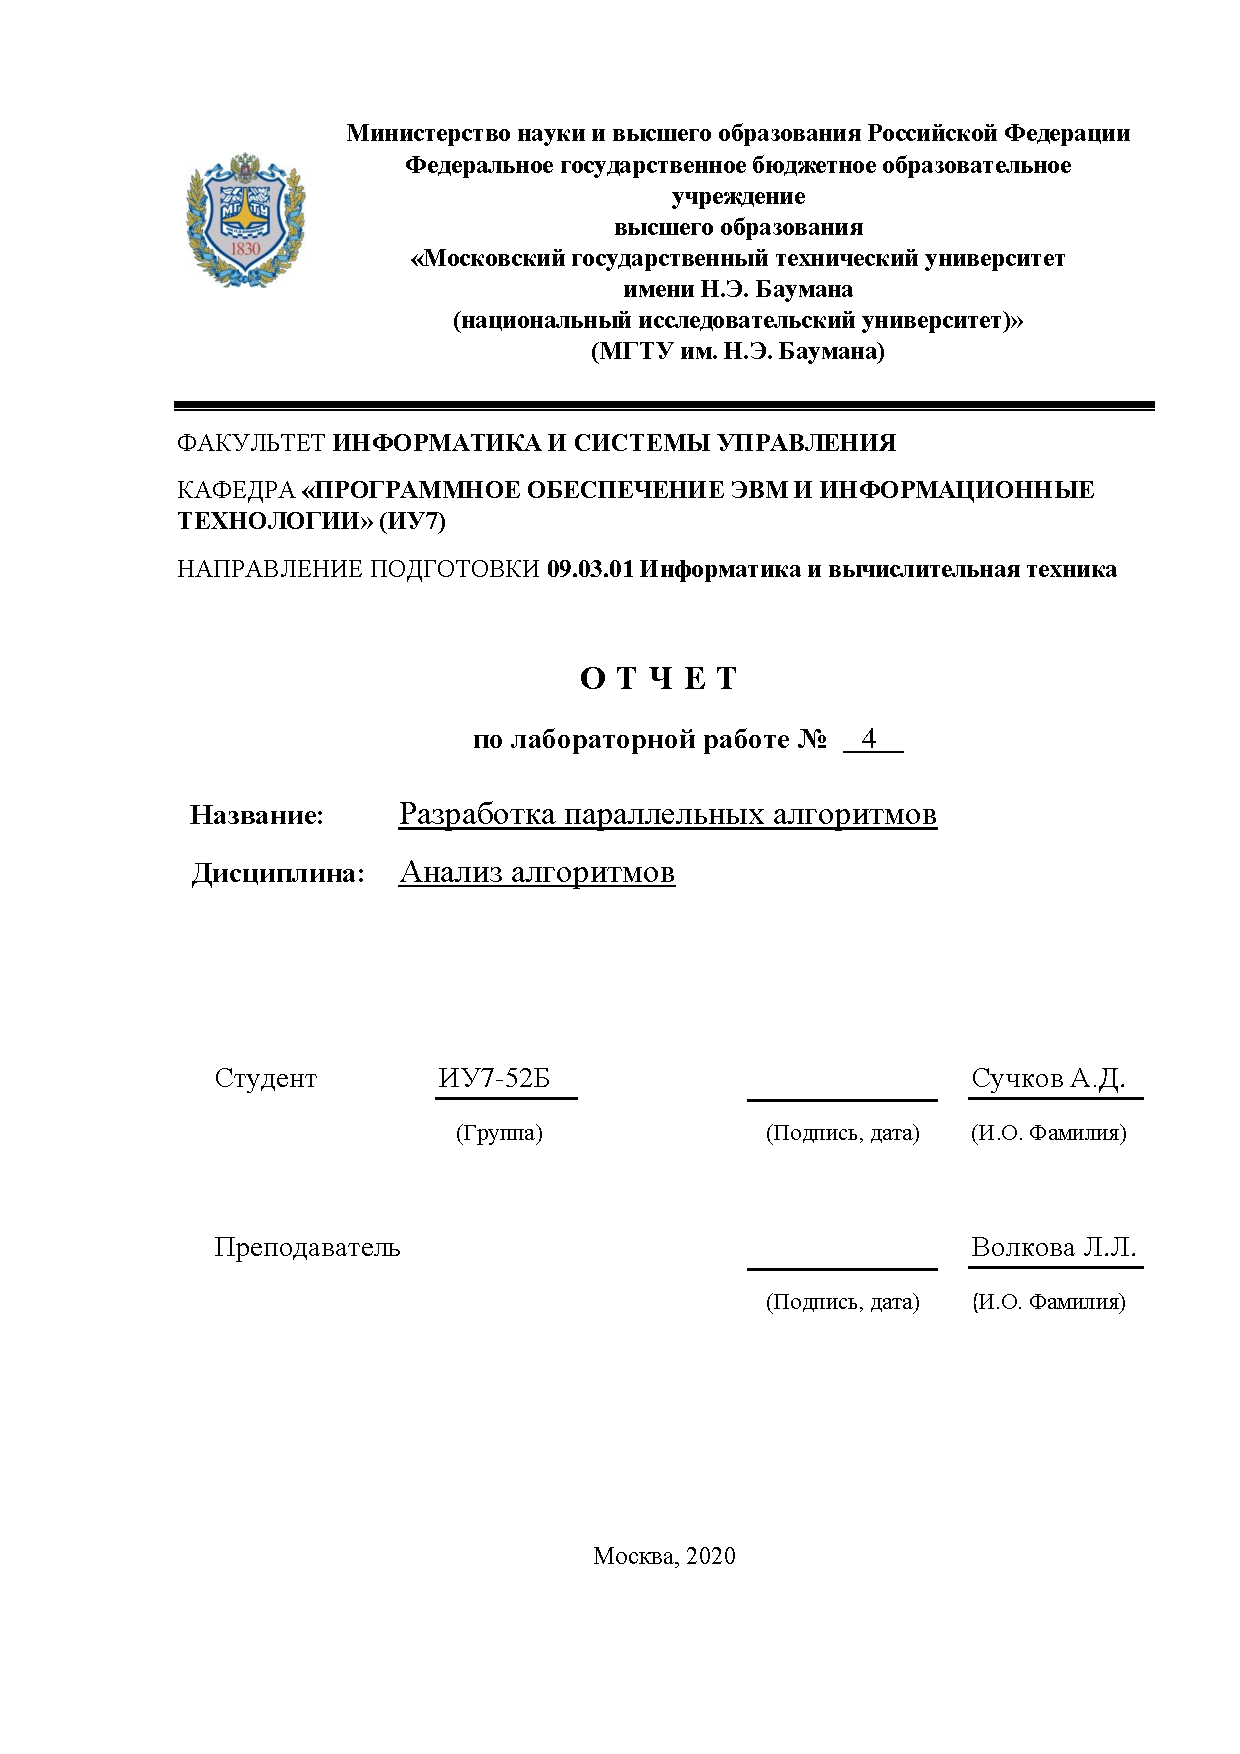
\includepdf[pages=1]{titul.pdf}
% Оглавление
\tableofcontents

\newpage
\chapter*{Введение}
\addcontentsline{toc}{chapter}{Введение}

В данной лабораторной работе реализуется и оценивается параллельный алгоритм классического умножения матриц.

Параллелизм -- выполнение нескольких вычислений в различных потоках. 
При параллельном программировании в процессоре с многоядерной архитектурой несколько процессов могут выполнятся 
одновременно на разных ядрах.
Это приводит к тому, что время выполнения параллельного алгоритма может быть ощутимо меньше, чем у его 
однопоточного аналога.

Стандартный алгоритм умножения матриц подразумевает проход по всем элементам результирующей матрицы C для 
вычисления их значений. Так как вычисление каждого элемента независимо, этот алгоритм подходит для реализации 
покоординатного параллелизма.

\newpage
\chapter{Аналитическая часть}

Целью лабораторной работы является разработка и исследование параллельных алгоритмов умножения матриц. \\

Можно выделить следующие задачи лабораторной работы:
\begin{itemize}
    \item описание понятия параллелизма и операции умножения матриц;
    \item описание и реализация непараллельного и двух параллельных версий алгоритма умножения матриц;
    \item проведение замеров процессорного времени работы алгоритмов при различном количестве потоков;
    \item анализ полученных результатов.
\end{itemize}

\section{Математическое описание операции умножения матриц}

Умножение матриц -- операция на матрицами $A[M * N]$ и $B[N * Q]$ \cite{belous_off}. 
Результатом операции является матрица C размерами M * Q, в которой каждый элемент $c_{i,j}$ задаётся 
формулой 1.1.

\begin{equation}
    c_{i,j} = \sum\limits_{k=1}^n (a_{i,k} \cdot b_{k,j})
    \label{formula:1}
\end{equation}

\section{Используемые алгоритмы}

Стандартный алгоритм подразумевает циклическое сложение всех элементов вышеописанной суммы для получения
каждого элемента матрицы C.

Параллелизм может быть достигнут за счёт выделения процессов, которые могут выполнятся независимо друг от 
друга.
В данном случае вычисление каждого элемента C ведётся независимо друг от друга, поэтому в качестве 
параллельных алгоритмов выбраны параллельное вычисление элементов строк и параллельное вычисление 
элементов столбцов.

\section{Вывод}

Результатом аналитического раздела стало определение цели и задач работы, описано понятие операции 
умножения матриц и описаны используемые алгоритмы.

\newpage
\chapter{Конструкторская часть}

В данном разделе рассмотрим описанные алгоритмы умножения матриц $A[M * N]$ и $B[N * Q]$ с результирующей 
матрицей умножения $C[M * Q]$.

\section{Стандартный алгоритм умножения}

Данный алгоритм непосредственно использует вышеприведённую формулу. 
Для вычисления каждого элемента матрицы C совершается циклический обход k элементов из таблиц A и B.

Схема алгоритма приведена на рисунке 2.1

\begin{figure}[h!]
    \center{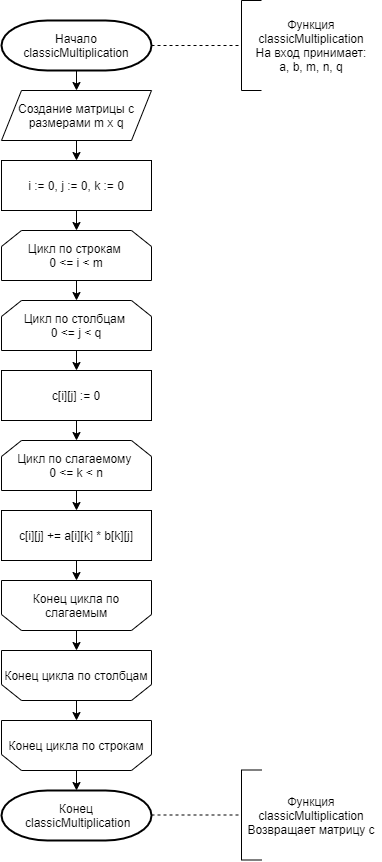
\includegraphics[scale=0.5]{schemes_classic.png}}
    \caption{Схема алгоритма классического умножения}
    \label{fig:image}
\end{figure}

\newpage
\section{Алгоритм умножения параллельный по строкам}

Вычисление каждого элемента матрицы является независимым. Поэтому возможна следующая параллельная 
реализация данного алгоритма. 

Пусть производится работа с T потоками. В таком случае, i-й поток будет производить вычисление строк
$i, i + T, i + 2T, \dots, ((M - i) mod T) \cdot T + i$.

Схема алгоритма приведена на рисунках 2.2 и 2.3

\begin{figure}[h!]
    \center{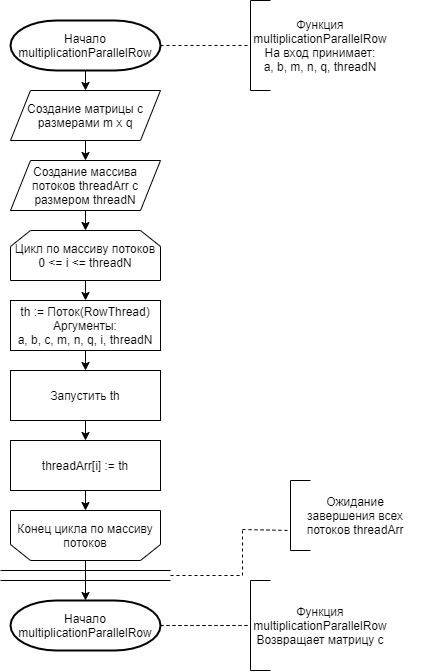
\includegraphics[scale=0.7]{schemes_parallel_row_1.png}}
    \caption{Схема алгоритма параллельного умножения по строкам, часть 1}
    \label{fig:image}
\end{figure}

\begin{figure}[h!]
    \center{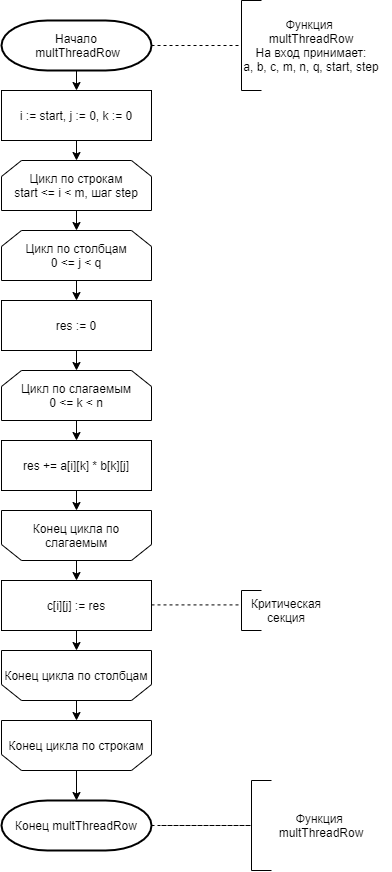
\includegraphics[scale=0.7]{schemes_parallel_row_2.png}}
    \caption{Схема алгоритма параллельного умножения по строкам, часть 2}
    \label{fig:image}
\end{figure} 

\section{Алгоритм умножения параллельный по столбцам}

В силу независимости вычислений каждого элемента, аналогично можно организовать и параллельное вычисление
значений в столбцах матрицы C. В таком случае, i-й поток будет производить вычисление столбцов
$i, i + T, i + 2T, \dots, ((Q - i) mod T) \cdot T + i$

Схема алгоритма приведена на рисунках 2.4 и 2.5

\begin{figure}[h!]
    \center{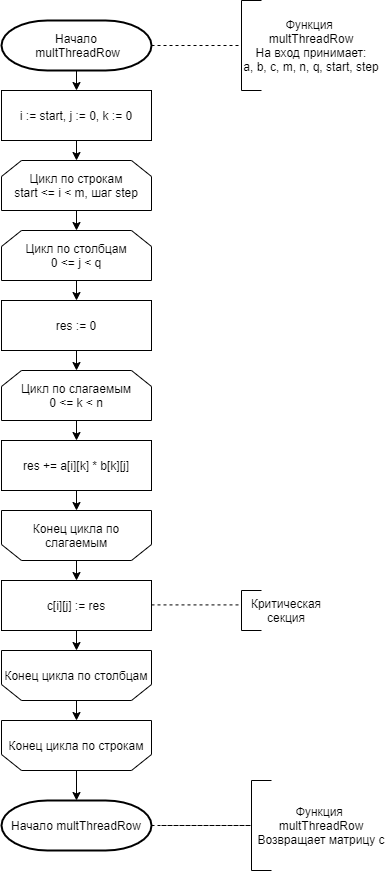
\includegraphics[scale=0.7]{schemes_parallel_col_1.png}}
    \caption{Схема алгоритма параллельного умножения по столбцам, часть 1}
    \label{fig:image}
\end{figure}

\begin{figure}[h!]
    \center{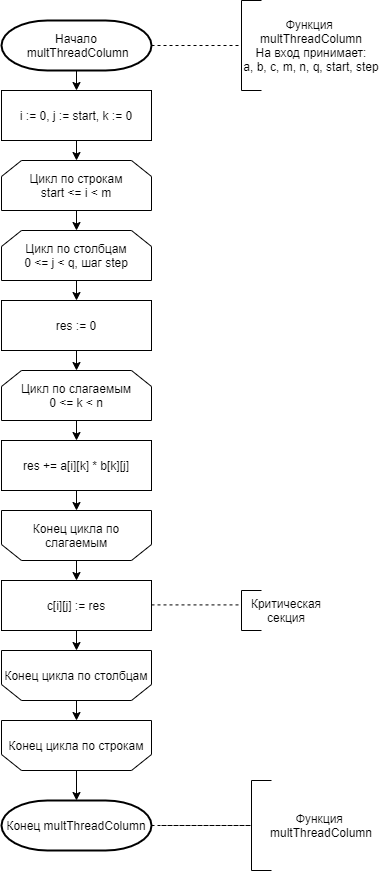
\includegraphics[scale=0.7]{schemes_parallel_col_2.png}}
    \caption{Схема алгоритма параллельного умножения по столбцам, часть 1}
    \label{fig:image}
\end{figure}

\newpage
\section{Требования к программному обеспечению}

Для полноценной проверки и оценки алгоритмов необходимо выполнить следующее:
\begin{figure}[h!]
    \begin{itemize}
        \item предоставить выбор алгоритма для умножения, обеспечить возможность консольного ввода двух 
        матриц и количества используемых потоков (в случае выбора многопоточного алгоритма). Программа 
        должна вывести результирующую матрицу.
        \item реализовать функцию замера процессорного времени, затраченного функциями.
    \end{itemize}
\end{figure}

\newpage
\section{Вывод}

Результатом конструкторской части стало схематическое описание алгоритмов умножения матриц, 
сформулированы тесты и требования к программному обеспечению.

\newpage
\chapter{Технологическая часть} 

\section{Выбор языка программирования}

В качестве языка программирования был выбран C++, так как имеется опыт работы с ним и с 
библиотеками, позволяющими провести исследование и тестирование программы. 
Также в языке имеются средства для использования многопоточности. 
Разработка проводилась в среде Visual Studio Code.

\section{Листинг кода}

В листингах 3.1 - 3.3 приведены реализации умножения матриц. \\

\textrm{Листинг 3.1: функция классического умножения матриц}
\begin{lstlisting}[frame=single, numbers=left]
matrixType classicMultiplication(matrixType a, 
                                 matrixType b, 
                                 int m, int n, int q)
{
    if (m != q)
        return;

    matrixType c = createMatrix(m, q);
    
    for (int i = 0; i < m; i++)
    {
        for (int j = 0; j < q; j++)
        {
            int res = 0;
    
            for (int k = 0; k < n; k++)
                res += a[i][k] * b[k][j];
    
            *(c + i * q + j) = res;
        }
    }
    return c;
}
\end{lstlisting}

\textrm{Листинг 3.2: функции параллельного умножения матриц по строкам}
\begin{lstlisting}[frame=single, numbers=left]
void multThreadRow(matrixType& c, matrixType& a, 
                   matrixType&b, int m, int n, 
                   int q, int start, int step)
{
    for (int i = start; i < m; i += step)
    {
        for (int j = 0; j < q; j++)
        {
            int res = 0;
    
            for (int k = 0; k < n; k++)
            {
                res += a[i][k] * b[k][j];
            }
            mtx.lock();
            *(c + i * q + j) = res;
            mtx.unlock();
        }
    }
}
    
matrixType multiplicationParallelRow(matrixType a, 
                                     matrixType b, 
                                     int m, int n, 
                                     int q, 
                                     int threadCnt)
{
    if (m != q)
        return;

    matrixType c = createMatrix(m, q);
    vector<thread> threadArray;
    
    for (int i = 0; i < threadCnt; i++)
    {
        threadArray.push_back(thread(multThreadRow, 
                                    ref(c), ref(a), 
                                    ref(b), m, n, q, 
                                    i, threadCnt));
    }
    
    for (int i = 0; i < threadCnt; i++)
    {
        threadArray[i].join();
    }
    
    return c;
}
\end{lstlisting}

\textrm{Листинг 3.3: функция параллельного умножения матриц по столбцам}
\begin{lstlisting}[frame=single, numbers=left]
void multThreadColumn(matrixType& c, matrixType& a, 
                      matrixType& b, int m, int n, 
                      int q, int start, int step)
{
    for (int i = 0; i < m; i++)
    {
        for (int j = start; j < q; j += step)
        {
            int res = 0;
    
            for (int k = 0; k < n; k++)
            {
                res += a[i][k] * b[k][j];
            }
    
            mtx.lock();
            *(c + i * q + j) = res;
            mtx.unlock();
        }
    }
}
    
matrixType multiplicationParallelColumn(matrixType a, 
                                        matrixType b, 
                                        int m, int n, 
                                        int q, 
                                        int threadCnt)
{
    if (m != q)
        return;

    matrixType c = createMatrix(m, q);
    vector<thread> threadArray;
    
    for (int i = 0; i < threadCnt; i++)
    {
        threadArray.push_back(thread(multThreadColumn, 
                                     ref(c), ref(a), 
                                     ref(b), m, n, q, 
                                     i, threadCnt));
    }
    
    for (int i = 0; i < threadCnt; i++)
    {
        threadArray[i].join();
    }
    return c;
}
\end{lstlisting}

\section{Результаты тестирования}

На рисунках 3.1 - 3.2 приведены скриншоты интерфейса программы и тестирования, которые проводились в ручную.

\begin{figure}[h!]
    \center{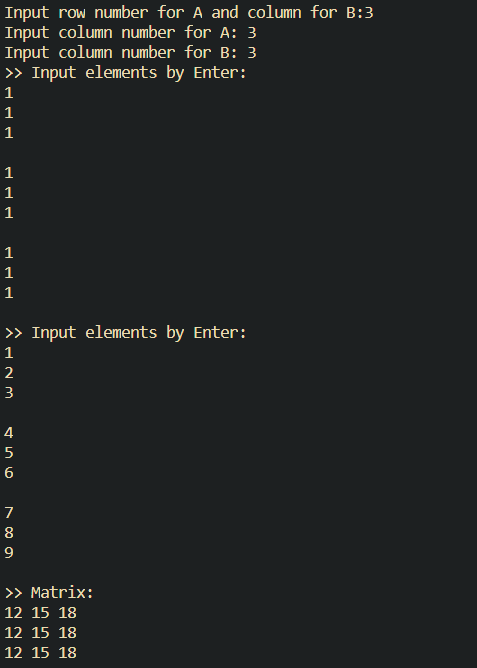
\includegraphics[scale=0.8]{../screen_1.png}}
    \caption{Пример 1}
    \label{fig:image}
\end{figure}

\begin{figure}[h!]
    \center{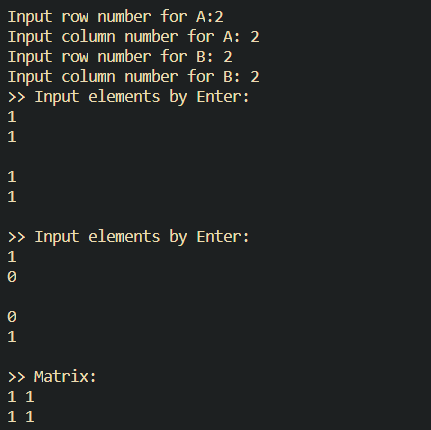
\includegraphics[scale=0.8]{../screen_2.png}}
    \caption{Пример 2}
    \label{fig:image}
\end{figure}

Все тесты прошли успешно.

\newpage
\section{Оценка времени}

Для замера процессорного времени исполнения функции используется функция 
QueryPerfomanceCounter библиотеки windows.h. 

Измерение производится в функциях, которые приведены в листинге 3.4.
Замеры времени на различных размерах матриц производятся в написанной
функции в листинге 3.5. \\

\textrm{Листинг 3.4: функции замера процессорного времени}
\begin{lstlisting}[frame=single, numbers=left]
double PCFreq = 0.0;
__int64 CounterStart = 0;
    
void StartCounter()
{
    LARGE_INTEGER li;
    if(!QueryPerformanceFrequency(&li))
    std::cout << "QueryPerformanceFrequency failed!\n";
    
    PCFreq = double(li.QuadPart);///1000.0;
    
    QueryPerformanceCounter(&li);
    CounterStart = li.QuadPart;
}
    
double GetCounter()
{
    LARGE_INTEGER li;
    QueryPerformanceCounter(&li);
    return double(li.QuadPart-CounterStart)/PCFreq;
}
\end{lstlisting}

\textrm{Листинг 3.5: функция замера времени на различных размерах матриц}
\begin{lstlisting}[frame=single, numbers=left]
void beginTimeTest()
{
    int countSize = 5;
    int sizes[] = { 32, 100, 250, 500, 1000 };
    
    char algorithmNames[][100] = {"Classic multiplication",
    "Parallel by row", "Parallel by column"};
    
    for (int i = 0; i < countSize; i++)
    {
        matrixType a = generateMatrix(sizes[i], sizes[i]);
        matrixType b = generateMatrix(sizes[i], sizes[i]);            
        double finishTime = 0;
    
        for (int j = 0; j < 5; j++)
        {
            StartCounter();
            classicMultiplication(a, b, sizes[i], 
                                sizes[i], sizes[i]);
            finishTime += GetCounter();
        }
    
        finishTime /= 5;
    
        cout << "\nFor " << algorithmNames[0] 
                        << "\t-> Row - " << sizes[i] 
                        << "\tColumn - " << sizes[i]
                        << "\tTime - " << finishTime;
        deleteMatrix(a, sizes[i]);
        deleteMatrix(b, sizes[i]);
    }
    
    matrixType (*algorithms[])(matrixType, matrixType, 
    int, int, int, int) = {multiplicationParallelRow, 
                        multiplicationParallelColumn};
    int p = 1;
    
    int nThreads[] = { 1, 2, 4, 8, 16, 32 };
    
    for (int k = 0; k < 2; k++)
    {
        matrixType (*mult)(matrixType, matrixType, 
                int, int, int, int) = algorithms[k];
    
        for (int i = 0; i < countSize; i++)
        {
            for (int threads = 0; threads < 6; threads++)
            {
                matrixType a = generateMatrix(sizes[i], 
                                              sizes[i]);
                matrixType b = generateMatrix(sizes[i], 
                                              sizes[i]);
    
                double finishTime = 0;
    
                for (int j = 0; j < 5; j++)
                {
                    StartCounter();
                    mult(a, b, sizes[i], sizes[i], 
                                         sizes[i], 
                                nThreads[threads]);
                    finishTime += GetCounter();
                }
    
                finishTime /= 5;
    
                cout << "\nFor " << algorithmNames[p] 
                            << "\t-> Row - " << sizes[i] 
                            << "\tColumn - " << sizes[i]
                            << "\tTime - " << finishTime;
    
                p++;
    
                deleteMatrix(a, sizes[i]);
                deleteMatrix(b, sizes[i]);
            }
        }
    }
}
\end{lstlisting}

\section{Вывод}

Результатом технологической части стал выбор используемых технических средств 
реализации и последующая реализация алгоритмов, системы тестов и замера 
времени работы на языке C++.

\chapter{Исследовательская часть} 

Измерения процессорного времени проводятся на квадратных матрицах c размерами: 
32, 100, 250, 500, 1000. Содержание матриц сгенерировано случайным образом.
Изучается серия экспериментов с количеством потоков 1, 2, 3, 4, 8, 16, 32.

Для повышения точности, каждый замер производится 5 раз, за конечный результат 
берётся среднее арифметическое.

\section{Результаты экспериментов}

Эксперименты проводились на компьютере со следующими характеристиками:
\begin{itemize}
    \item ОС - Windows 10, 64bit;
    \item Процессор - Intel Core i5 7300HQ 2.5GHz, 4 Core 8 Logical Processor
    \item ОЗУ - 8Gb
\end{itemize}

По результатам измерений процессорного времени можно составить таблицы 4.1 - 4.5.

\begin{table}[h!]
\caption{Результаты замеров процессорного времени при размере 32 (в миллисекундах)}
\label{tabular:timesandtenses}
\begin{center}
\begin{tabular}{ | l | l | l | l | l | l | l | }
\hline
        Потоки                   & 1    & 2    & 4    & 8    & 16   & 32   \\ \hline
        Многопоточно по строкам  & 0.24 & 0.29 & 0.36 & 0.58 & 1.04 & 2.02 \\ \hline
        Многопоточно по столбцам & 0.24 & 0.30 & 0.35 & 0.59 & 1.03 & 1.97 \\ \hline
        Однопоточно              &      \multicolumn{5}{c}{0.096}   &      \\ \hline
\end{tabular}
\end{center}
\end{table}

\begin{table}[h!]
\caption{Результаты замеров процессорного времени при размере 100 (в миллисекундах)}
\label{tabular:timesandtenses}
\begin{center}
\begin{tabular}{ | l | l | l | l | l | l | l | }
\hline
        Потоки                   & 1    & 2    & 4    & 8    & 16   & 32   \\ \hline
        Многопоточно по строкам  & 5.52 & 2.73 & 2.80 & 2.78 & 3.09 & 3.51 \\ \hline
        Многопоточно по столбцам & 4.87 & 3.14 & 2.87 & 2.89 & 3.15 & 3.57 \\ \hline
        Однопоточно              &      \multicolumn{5}{c}{2.96}    &      \\ \hline
\end{tabular}
\end{center}
\end{table}

\begin{table}[h!]
\caption{Результаты замеров процессорного времени при размере 250 (в секундах)}
\label{tabular:timesandtenses}
\begin{center}
\begin{tabular}{ | l | l | l | l | l | l | l | }
\hline
        Потоки                   & 1     & 2     & 4     & 8     & 16    & 32    \\ \hline
        Многопоточно по строкам  & 0.068 & 0.042 & 0.031 & 0.024 & 0.026 & 0.024 \\ \hline
        Многопоточно по столбцам & 0.064 & 0.047 & 0.035 & 0.027 & 0.034 & 0.030 \\ \hline
        Однопоточно              &       \multicolumn{5}{c}{0.051}       &       \\ \hline
\end{tabular}
\end{center}
\end{table}

\begin{table}[h!]
\caption{Результаты замеров процессорного времени при размере 500 (в секундах)}
\label{tabular:timesandtenses}
\begin{center}
\begin{tabular}{ | l | l | l | l | l | l | l | }
\hline
        Потоки                   & 1    & 2    & 4    & 8    & 16   & 32   \\ \hline
        Многопоточно по строкам  & 0.61 & 0.38 & 0.26 & 0.20 & 0.21 & 0.20 \\ \hline
        Многопоточно по столбцам & 0.62 & 0.42 & 0.28 & 0.23 & 0.24 & 0.24 \\ \hline
        Однопоточно              &     \multicolumn{5}{c}{0.051}    &      \\ \hline
\end{tabular}
\end{center}
\end{table}

\begin{table}[h!]
\caption{Результаты замеров процессорного времени при размере 1000 (в секундах)}
\label{tabular:timesandtenses}
\begin{center}
\begin{tabular}{ | l | l | l | l | l | l | l | }
\hline
        Потоки                   & 1    & 2    & 4    & 8    & 16   & 32   \\ \hline
        Многопоточно по строкам  & 8.22 & 4.63 & 2.64 & 2.18 & 2.22 & 2.27 \\ \hline
        Многопоточно по столбцам & 8.33 & 5.64 & 3.05 & 2.62 & 2.82 & 2.89 \\ \hline
        Однопоточно              &     \multicolumn{5}{c}{7.13}     &      \\ \hline
\end{tabular}
\end{center}
\end{table}

\newpage
\section{Вывод}

По результатам экспериментов можно заключить следующее:
\begin{itemize}
    \item при относительно небольшом размере матриц (менее 100x100) использование потоков для 
    уменьшения времени исполнения нецелесообразно, так как накладные расходы времени на 
    управление потоками и mutex-ами больше, чем выигрыш от параллельного выполнения выполнения
    вычислений;
    \item использование по крайней мере двух потоков даёт ощутимый выигрыш по времени по 
    сравнению с однопоточной версией алгоритма;
    \item использование одного потока в многопоточных версиях алгоритма проигрывает по времени
    по сравнению с однопоточной версией алгоритма, что объясняется накладными расходами времени
    на управление потоками и mutex-ами;
    \item использование 16 и 32 потоков показывает результат по времени несколько хуже, чем при 
    8 потоках, из чего следует, что увеличение потоков даёт выигрыш по времени лишь до достижения
    определённого количества, так как появляются большие накладные затраты по времени для 
    управления большим количеством потоков и mutex-ов;
    \item параллельные версии алгоритма выполняются за приблизительно одинаковое время при одном
    потоке. Однако, использование большего количества потоков выявляет, что многопоточность по 
    строкам быстрее многопоточности по столбцам вплоть до 20\%;
    \item наиболее быстродейственно алгоритм действует на 8 потоках, что равно количеству 
    логических процессоров на испытуемом компьютере.
\end{itemize}

\newpage
\chapter*{Заключение}
\addcontentsline{toc}{chapter}{Заключение} 

В ходе лабораторной работы достигнута поставленная цель: разработка и исследование параллельных
алгоритмов умножения матриц.
Решены все задачи.

Были изучены и описаны понятия параллелизма и операции умножения матриц.
Также были описан и реализованы непараллельный и две параллельные реализации алгоритма умножения
матриц.
Проведены замеры процессорного времени работы алгоритмов при различном количестве потоков.
На основании экспериментов проведён сравнительный анализ.

Из проведённых экспериментов было выявлено, что наиболее быстродеиственным является использование
количество потоков, которое совпадает с количеством логических процессоров процессора. 
Увеличение или уменьшение количества потоков ведёт к большему времени выполнения вычислений.
Однако, использование потоков даёт выигрыш по времени работы только для относительно больших
размеров матриц, иначе их использование лишь увеличит время вычислений за счёт накладных
расходов.
Также было установлено, что алгоритм, использующий многопоточность по строкам показывает себя
несколько быстрее алгоритма с многопоточностью по столбцам.

\newpage
\renewcommand\bibname{Список литературы}
\addcontentsline{toc}{chapter}{Список литературы}
\makeatletter % список литературы
\def\@biblabel#1{#1. }
\makeatother
\begin{thebibliography}{2}
    \bibitem{cpp_info} Документация языка C++ 98 [Электронный ресурс], режим доступа: http://www.open-std.org/JTC1/SC22/WG21/, свободный (дата обращения: 14.10.20202).
    \bibitem{belous_off} Белоусов И. В. МАТРИЦЫ И ОПРЕДЕЛИТЕЛИ: учебное пособие по линейной алгебре. / Кишинев: 2006/.
\end{thebibliography}

\end{document}